\section{Analytic Solution: Log Utility Case ($\psi = \gamma = 1$)}\label{sec:log_utility.sec} % SB: we had mentioned this special case already.

Here, we consider log utility. This case is special because, as we show next, the LDF is only a function of market beliefs. % as opposed to what? 
For this case, we derive a law of motion for market beliefs which renders sharp predictions about how belief heterogeneity amplifies business cycles. We return to a general class of preferences in the quantitative section that follows this one.

\paragraph{Equilibrium Labor Demand Factor Given Market Beliefs.}

Under log utility, the consumption-wealth ratio and portfolio shares specialize to:
\begin{equation}\nonumber
    c_i(X) = 1-\beta, \qquad \qquad 
    \omega_{i}(X,s) = \frac{1}{\Delta R_r(X,s)} \left[\frac{p_{sH}^i}{p_{sH}\Lambda(X,s,H)}  -\frac{p_{sL}^i}{p_{sL}\Lambda(X,s,L)} \right].
\end{equation}
% Under log utility---$\psi = \gamma = 1$, income and substitution effects cancel out from portfolio decisions, Proposition XXX specialize to:\todo{add prop #.} 
% \todo{what about presenting the formulas with ratios of square roots? Seems cleaner.}
% \begin{equation}\nonumber
%     c_i(X) = 1-\beta, \qquad \qquad 
%     \sigma_s[R_{i,n}(X,s,s')] = \sqrt{p_{sL} p_{sH}} \left[\frac{p_{sH}^i}{p_{sH}\Lambda(X,s,H)}  -\frac{p_{sL}^i}{p_{sL}\Lambda(X,s,L)} \right],
% \end{equation}
% where $\sigma_s[R_{i,n}(X,s,s')] = \omega_{i}(X,s) \sigma_s[R_{r}(X,s,s')]$.
Combined with the market clearing conditions \eqref{eq: mkt_clearing_markov}, they yield the risk-free rate and the risk premium. 
\begin{proposition}[Risk-free rate and risk premium] \label{prop: asset_prices} Given $\mathcal{L}'(X,s)$
\begin{enumerate}[(i)]
    \item The risk-free rate is 
    \begin{equation}
        R_{b}(X,s) = \left(1 - \frac{\alpha}{1+\nu}\right)\frac{x_s}{\beta} \frac{ \mathcal{L}'(X,s)^{\frac{1+\nu}{1+\nu-\alpha}}}{x_{s} \mathcal{L}^\frac{\alpha}{1+\nu-\alpha} - \frac{\alpha}{1+\nu} \mathcal{L}^{\frac{1+\nu}{1+\nu-\alpha}} }.
    \end{equation}
    \item The conditional risk premium is given by
    %SB: too mucho\footnote{We are focusing on the risk premium computed using the objective measure. 
    %Alternatively, we can define $\mathbb{E}_s^i[R_{p}^e(X,s,s')]$, the expected excess return computed with investor $i$ beliefs, which would be given by an expression analogous to \eqref{eq: risk_premium}, but with $\mathbb{E}_s^i[x_{s'}]$ in the place of $\mathbb{E}_s[x_{s'}]$.
    
    \begin{equation}\label{eq: risk_premium}
    \mathbb{E}_s[R_{r}^e(X,s,s')] = \frac{1}{1 - \frac{\alpha}{1+\nu}} \frac{\mathbb{E}_s[x_{s'}] - \mathcal{L}'(X,s)}{\mathcal{L}'(X,s)}.
    % \mathbb{E}_s[R_{r}^e(X,s,s')] = \frac{x_s}{\beta} \frac{(\mathbb{E}_s[x_{s'}] - E'(X,s))E'(X,s)^\frac{\alpha}{1+\nu-\alpha}}{x_{s} E^\frac{\alpha}{1+\nu-\alpha} - \frac{\alpha}{1+\nu} E^{\frac{1+\nu}{1+\nu-\alpha}} }.
\end{equation}
    $\mathbb{E}_s[R_{r}^e(X,s,s')]$ is decreasing in $\mathcal{L}'(X,s)$.
\end{enumerate}
\end{proposition}
\begin{proof}
See Appendix \ref{app: proof_asset_prices}.
\end{proof}
Proposition \ref{prop: asset_prices} shows that the risk-free rate and the risk premium can be deduced from the current productivity growth, $x_s$, and the lagged and current period's LDF, $\mathcal{L}$ and $\mathcal{L}'(X,s)$. The risk free rate, $R_{b}(X,s)$, is increasing in $\mathcal{L}'(X,s)$ and decreasing in $x_s$ whereas the risk premium $\mathbb{E}_s[R_{r}^e(X,s,s')]$ moves in the opposite direction. Ceteris paribus, periods of low-risk premium are associated with a high labor demand. 
%s with labor demand conditions: an increase of $\mathcal{L}'(X,s)$ leads to a decline in the risk premium but leads to an increase in the risk-free rate. 


Of course, the LDF $\mathcal{L}'(X,s)$ is endogenous and a function of market beliefs. 
Next, we solve for the equilibrium LDF by translating the market clearing conditions into a demand and supply system, where the quantity variable is the risk in investors' portfolios. Once risk is determined, we recover the LDF and all asset prices.

The demand and supply of risk are a convenient transformation of the asset-market clearing conditions \eqref{eq: mkt_clearing_markov}: multiply both sides of the condition for risky assets by $\sigma_s[R_r(X,s,s')]$, and use that $\sigma_s[R_{i,n}(X,s,s')] = \omega_{i}(X,s) \sigma_s[R_{r}(X,s,s')]$, to obtain:
\begin{equation*}
    \underbrace{\sum_{i=1}^I \eta_i \sigma_s[R_{i,n}(X,s,s')]}_{\text{demand for risk}} =  \underbrace{\sigma_s[R_r(X,s,s')]}_{\text{supply of risk}}.
\end{equation*}
The left of the expression is the \textit{demand for risk}.  The demand for risk corresponds is the volatility of total wealth that households needed to guarantee asset market clearing at given asset prices.
The right-hand side represents the \textit{supply of risk}. The supply of risk is the volatility of the economy's surplus claim induced by the firm's labor demand at given asset prices. The next proposition expresses the demand and supply of risk as a function of the LDF.
 
%As shown in Proposition \ref{prop: E_sharpe}, the risk-neutral expectation of productivity is tightly connected to the price of risk, as an increase in the Sharpe ratio of the risky asset reduces the value of $E'(X,s)$. In turn, the price of risk, and ultimately $E'(X,s)$, are determined by a notion of demand for risk (or risk appetite) and the supply a risk, as we explain in the following proposition. 
\begin{proposition}[The demand and supply of risk] \label{prop: risk} Suppose $x_L > \alpha x_H $. Then,
\begin{enumerate}[(i)]
    \item The supply of risk is
    \begin{equation}
        \sigma_s[R_r(X,s,s')] = \frac{x_s}{\beta} \frac{\sigma_s[x_{s'}] \mathcal{L}'(X,s)^\frac{\alpha}{1+\nu-\alpha}}{x_{s} \mathcal{L}^\frac{\alpha}{1+\nu-\alpha} - \frac{\alpha}{1+\nu} \mathcal{L}^{\frac{1+\nu}{1+\nu-\alpha}} }.
    \end{equation}
    
    % SB: commented out because paper is very dense. 
    \item The demand for risk is
    \begin{equation}
        \sum_{i=1}^I \eta_i \sigma_s[R_{i,n}(X,s,s')] =  \sigma_s[x_{s'}] R_b(X,s) \left[\frac{\overline{p}^m_{sH}(X)}{\mathcal{L}'(X,s) - x_L}  -\frac{\overline{p}^m_{sL}(X)}{x_H-\mathcal{L}'(X,s)} \right],
    \end{equation}
    where $\overline{p}_{ss'}^{m}(X) \equiv \sum_{i=1}^I \eta_i p_{ss'}^i$.
\end{enumerate}

\end{proposition}
\begin{proof}
See Appendix \ref{app: proof_risk}.
\end{proof}
Proposition \ref{prop: risk} implies that the supply of risk is increasing in $\mathcal{L}'(X,s)$, while the demand for risk is decreasing in $\mathcal{L}'(X,s)$, as shown in Figure \ref{fig: risk_eq}. As with any demand system, the equilibrium $\mathcal{L}'(X,s)$ falls in the intersection. 
% Observe that Proposition \ref{prop: risk} implies that the supply of risk is increasing in $E'(X,s)$ and decreasing in $x_s$. The demand of risk is decreasing in $E'(X,s)$ and $x_s$, and increasing in $p_{sH}(X,s)$, where $p_{ss'}(X) = \sum_{i=1}^I \eta_{i,t} p_{ss'}^i$. 

% These curves correspond to the left-hand side and right-hand side of asset-market clearing condition (xxx). We interpret the right hand side as the supply of risk, and the left-hand side as the supply. 
Let's delve into the supply of risk. The risk of the surplus claim increases in $\mathcal{L}'(X,s)$ through an \textit{operating leverage channel}.\footnote{
Operating leverage is the ratio of revenues minus contemporary variable costs (zero in our setting) to profits. 
The relation between return risk and operating leverage originally appears in \citet{lev1974association}. 
For evidence on this channel, see e.g. \citet{novy2010operating} and \citet{donangelo2019cross}.} 
% Why? 
Recall that labor demand increases with $\mathcal{L}'(X,s)$. Because labor is hired in advance, costs are fixed while revenues are risky. Thus, there is more risk with a greater LDF, $\mathcal{L}'(X,s)$, as the following formula demonstrates:
\begin{equation}\label{eq: coef_variation_returns}
    \frac{\sigma_s[R_r(X,s,s')]}{\mathbb{E}_s[R_r(X,s,s')]} = \frac{\sigma_s[x']}{\mathbb{E}_s[x_{s'}]} \underbrace{\frac{\mathbb{E}_s[x_{s'}] \mathcal{L}'(X,s)^\frac{\alpha}{1+\nu-\alpha} }{\mathbb{E}_s[x_{s'}] \mathcal{L}'(X,s)^\frac{\alpha}{1+\nu-\alpha} - \frac{\alpha}{1+\nu} \mathcal{L}'(X,s)^{\frac{1+\nu}{1+\nu-\alpha}} }}_{\text{operating leverage}} > \frac{\sigma_{s}[x_{s'}]}{\mathbb{E}_s[x_{s'}]}.
\end{equation}
In words, the risk in the aggregate surplus is an amplified version of the underlying risk, $\frac{\sigma_{s}[x_{s'}]}{\mathbb{E}_s[x_{s'}]}$, where the amplification factor is the operating leverage. Through this amplification, actual earnings are also more volatile than consumption, as in the data.\footnote{If labor were chosen after productivity is known, dividends and consumption would be equally volatile. With preset labor, TFP shocks disproportionately impact dividends. A pattern of more volatile dividends than consumption is consistent with the data  (see e.g. \citealt{campbell2003consumption}), but, thus, inconsistent with models in which there is no risk in hiring.} 
% Furthermore, the formula also implies that the supply of risk decreases with $x_s$. This means that risk is higher in during downturns, also as in the data.\todo{Refs? not sure we can make the claim because the claim is about states, not about x holding fixed E.}  
%All in all, since the supply of risk stems from the firm's hiring decision, it increases in the expectation $E'(X,s)$.

Let's turn to the demand for risk. 
The demand for risk is decreasing in $\mathcal{L}'(X,S)$.
As shown in Proposition \ref{prop: asset_prices}, the risk premium is inversely related to $\mathcal{L}'(X,S)$, so
investors are more willing to hold risky assets when the risk premium is high. 
The demand for risk is itself a function of \textit{market beliefs}, a weighted average of investors' beliefs, $\overline{p}_{ss'}^m(X)$.
As market beliefs become more optimistic, investors are willing to hold more risky assets for a given level of risk premium.
% The demand for risk is then consistent with the idea that more optimistic markets increase the demand for risky assets.
% This makes sense. It tells us that if market beliefs are more optimistic, this leads to an increase in the demand for risky assets.

\begin{figure}[t!]
    \centering
            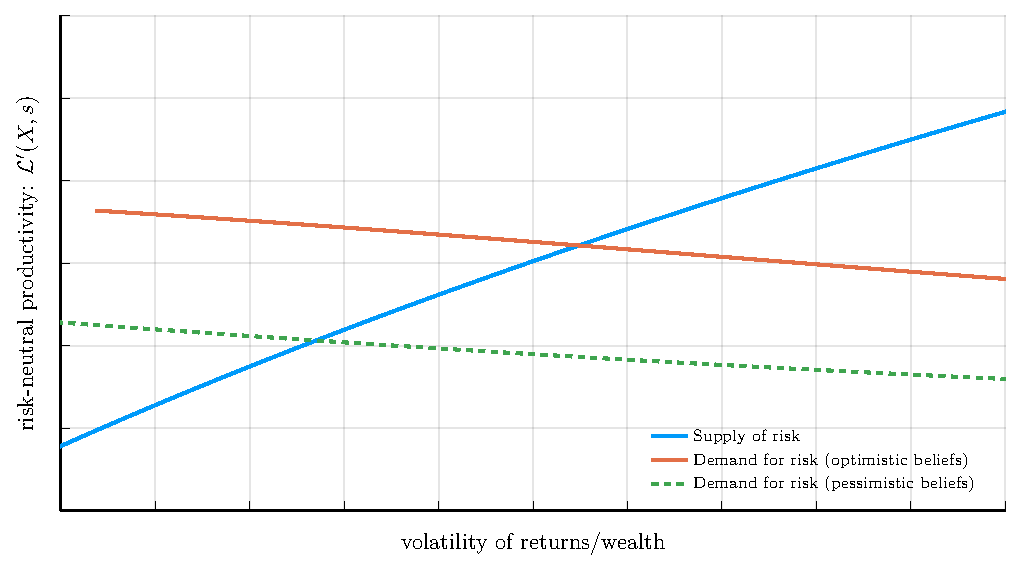
\includegraphics[width=0.7\textwidth]{figures/risk_equilibrium_inv.pdf}
    \caption{Equilibrium in the market for risky assets}
    \vspace{0.0cm}
    \label{fig: risk_eq}
\end{figure}
Propositions \ref{prop: asset_prices} and \ref{prop: risk} demonstrate that, unlike models where hiring occurs after productivity is realized, %here, 
labor demand and asset prices are determined jointly. 
We combine the demand and supply for risk to obtain the equilibrium LDF as a function of current market beliefs. 
\begin{corollary}[Labor demand factor]\label{cor: Eprime} The risk-neutral expectation of productivity growth $\mathcal{L}'(X,s)$ corresponds to the smallest real root of the quadratic equation: 
\begin{equation}
    \frac{\alpha}{1+\nu} \mathcal{L}'(X,s)^2  - \left[ \overline{p}^m_{sH}(X) \left(x_L + \frac{\alpha}{1+\nu}x_H \right)+ \overline{p}^m_{sL}(X)\left( \frac{\alpha}{1+\nu} x_L + x_H \right) \right] \mathcal{L}'(X,s) + x_L x_H = 0.\nonumber
\end{equation}
\end{corollary}
\begin{proof}
See Appendix \ref{app: proof_risk}.
\end{proof}
% This corollary shows that, for the log case, the LDF is determined statically by market beliefs, independently of the state variables affect current or future production.
The corollary shows that, for the log case, the LDF is independent of the current state $s$. The LDF is only a function of market beliefs. The wealth distribution affects asset prices and labor decisions to the extent it affects market beliefs wich are, in turn, a wealth-weighted average of underlying beliefs.
An important implication is that with homogeneous beliefs that states are i.i.d., hours are constant. Because productivity growth is close to i.i.d. under the objective measure, this result indicates the importance of non-rational beliefs in generating business cycle fluctuations.

Figure \ref{fig: risk_eq} also illustrates how we can exploit this demand system representation to explain the effects of changes in market beliefs: When market beliefs are pessimistic, there is a decline in the demand for risk, which leads to a decrease in the equilibrium LDF and, ultimately, a drop in hours. 
% As discussed above, the reduction in production caused by pessimism does not require firm managers to be pessimistic. It requires that managers reduce their labor demand to avoid depressing the firm value when markets become more pessimistic. 
% For instance, when market beliefs are more pessimistic, there is a decline in the demand for risk proving a decrease in the equilibrium LDF, which ultimately leads to a drop in hours. 

%\footnote{This channel is analogous to how changes in the cost of capital, the sum of the interest rate and the firm's risk premium, affects investment decisions.
%The key difference is that the costs and benefits of hiring an additional worker are incurred at the same time, so it is the risk premium, instead of the cost of capital, that affects the hiring decision.
%}

\paragraph{From the LDF to the Evolution of Market Beliefs.}

Corollary \ref{cor: Eprime} shows that given market beliefs, we can compute the LDF and asset prices. Another convenient property of log preferences is that the law of motion of market beliefs and wealth, has an analytic representation:
\begin{proposition}[Dynamics of wealth and market beliefs]\label{prop: dynamics_beliefs} Let $\psi = \gamma = 1$. Then,
\begin{enumerate}[(i)]
    \item the wealth share of investor $i\in \mathcal{I}$ evolves as:
    \begin{equation}
    \eta_i'(X,s,s') = \eta_i \frac{p^i_{ss'}}{\overline{p}^m_{ss'}(X)},
\end{equation}

    \item market beliefs are:
    \begin{equation}
        \overline{p}^m_{s'H}(X') = \sum_{i=1}^I \eta_i \frac{p^i_{ss'}}{\overline{p}^m_{ss'}(X)} p_{s'H}^i.
    \end{equation}
\end{enumerate}
\end{proposition}
\begin{proof}
See Appendix \ref{app: proof_dynamics_beliefs}.
\end{proof}
\todo{change to market beliefs here...}
Proposition \ref{prop: dynamics_beliefs} shows that the wealth of household $i$ increases when it assigns a greater likelihood to the realized state than what market beliefs do. Next, we present a taxonomy of belief types. The analytic representation in Corollary \ref{cor: Eprime} and Proposition \ref{prop: dynamics_beliefs} provides a tool to uncover how beliefs impact business cycles.


\subsection{Belief Taxonomy and Business Cycle Properties}

We classify belief structures and show how each has different business cycle implications. We provide the following taxonomy: 
\begin{definition}[Taxonomy of beliefs] Household $i$ is optimistic (pessimistic) relative to a benchmark belief $o$ at state $s$ if $p_{sH}^i > p_{sH}^o$ ($p_{sH}^i > p_{sH}^o$). We further classify belief structures:
\begin{enumerate}[(i)]
    \item Beliefs are \textbf{rank preserving}  if $i$ is optimistic or pessimistic relative to $o$, $\forall s$.
    \item Beliefs are \textbf{rank alternating}  if $i$ is optimistic relative to $o$ in one state, but $i$ is pessimistic relative to $o$ in the other state. 
\end{enumerate}
\end{definition}
Under this definition, the index $o$ represents a belief benchmark: it can be another household's belief or rational beliefs. We exploit this taxonomy to show that different belief structures induce different business cycle amplification properties, both in terms of the amplitude and the phase of the business cycle. 
%irst, we investigate the different predictions under homogeneous non-rational beliefs.
%We then discuss how heterogeneous non-rational beliefs produces internal propagation mechanism and discuss the different properties of different belief structures.

\paragraph{Homogeneous beliefs.}
With homogeneous beliefs, we have a representative investor. Hence, the model lacks internal propagation: the LDF only depends on the current state, $x_s$.
Furthermore, as noted above, if investors believe that productivity growth is iid, $p_{LH}(X) = p_{HH}(X)$, then the LDF and, thus, hours are constant. 

Away from iid growth,\todo{beliefs or growth} beliefs may amplify or dampen cycles relative to a rational expectations benchmark. Figure \ref{fig: hom_beliefs} illustrate this point. The figure simulates four periods of recession within a twenty-period interval for five types of homogeneous belief classifications: rational expectations $(p_{ss'}^i = p_{ss'}$ for all $s,s'$); two rank-preserving cases: always optimistic $(p_{sH}^i > p_{sH}$ for all $s$) or consistently pessimistic $(p_{sH}^i < p_{sH}$ for all $s$); and two rank-alternating cases: extrapolative $(p_{ss'}^i > p_{s s'}$ all $s=s')$ defined as optimistic during booms but pessimistic at busts, and intrapolative $(p_{ss'}^i < p_{ss'}$ all $s = s'$) defined as pessimistic at booms but pessimistic at busts.

Among rank-preserving beliefs: optimistic beliefs amplify expansions but dampen recessions relative to rational expectations. The converse is true about pessimistic beliefs: recessions are amplified and expansions dampened. All in all, rank-preserving beliefs have state-dependent amplification properties. Rank-alternating beliefs operate differently. Recall that extrapolative beliefs alternate, being optimistic at good states but pessimistic at bad states. Under extrapolative beliefs, the cycle's amplitude is magnified. Analogously, intrapolative beliefs produce the opposite: they reduce the cycle's amplitude. In conclusion, extrapolative beliefs are the belief structure that amplifies the cycle relative to rational expectations.
\todo{Note that Harrison-Kreps doesn't necessarily amplify the cycle because it depends on who makes money. It could dampen the cycle...Would like to build a connection here.}

\begin{figure}[t!]
    \centering
            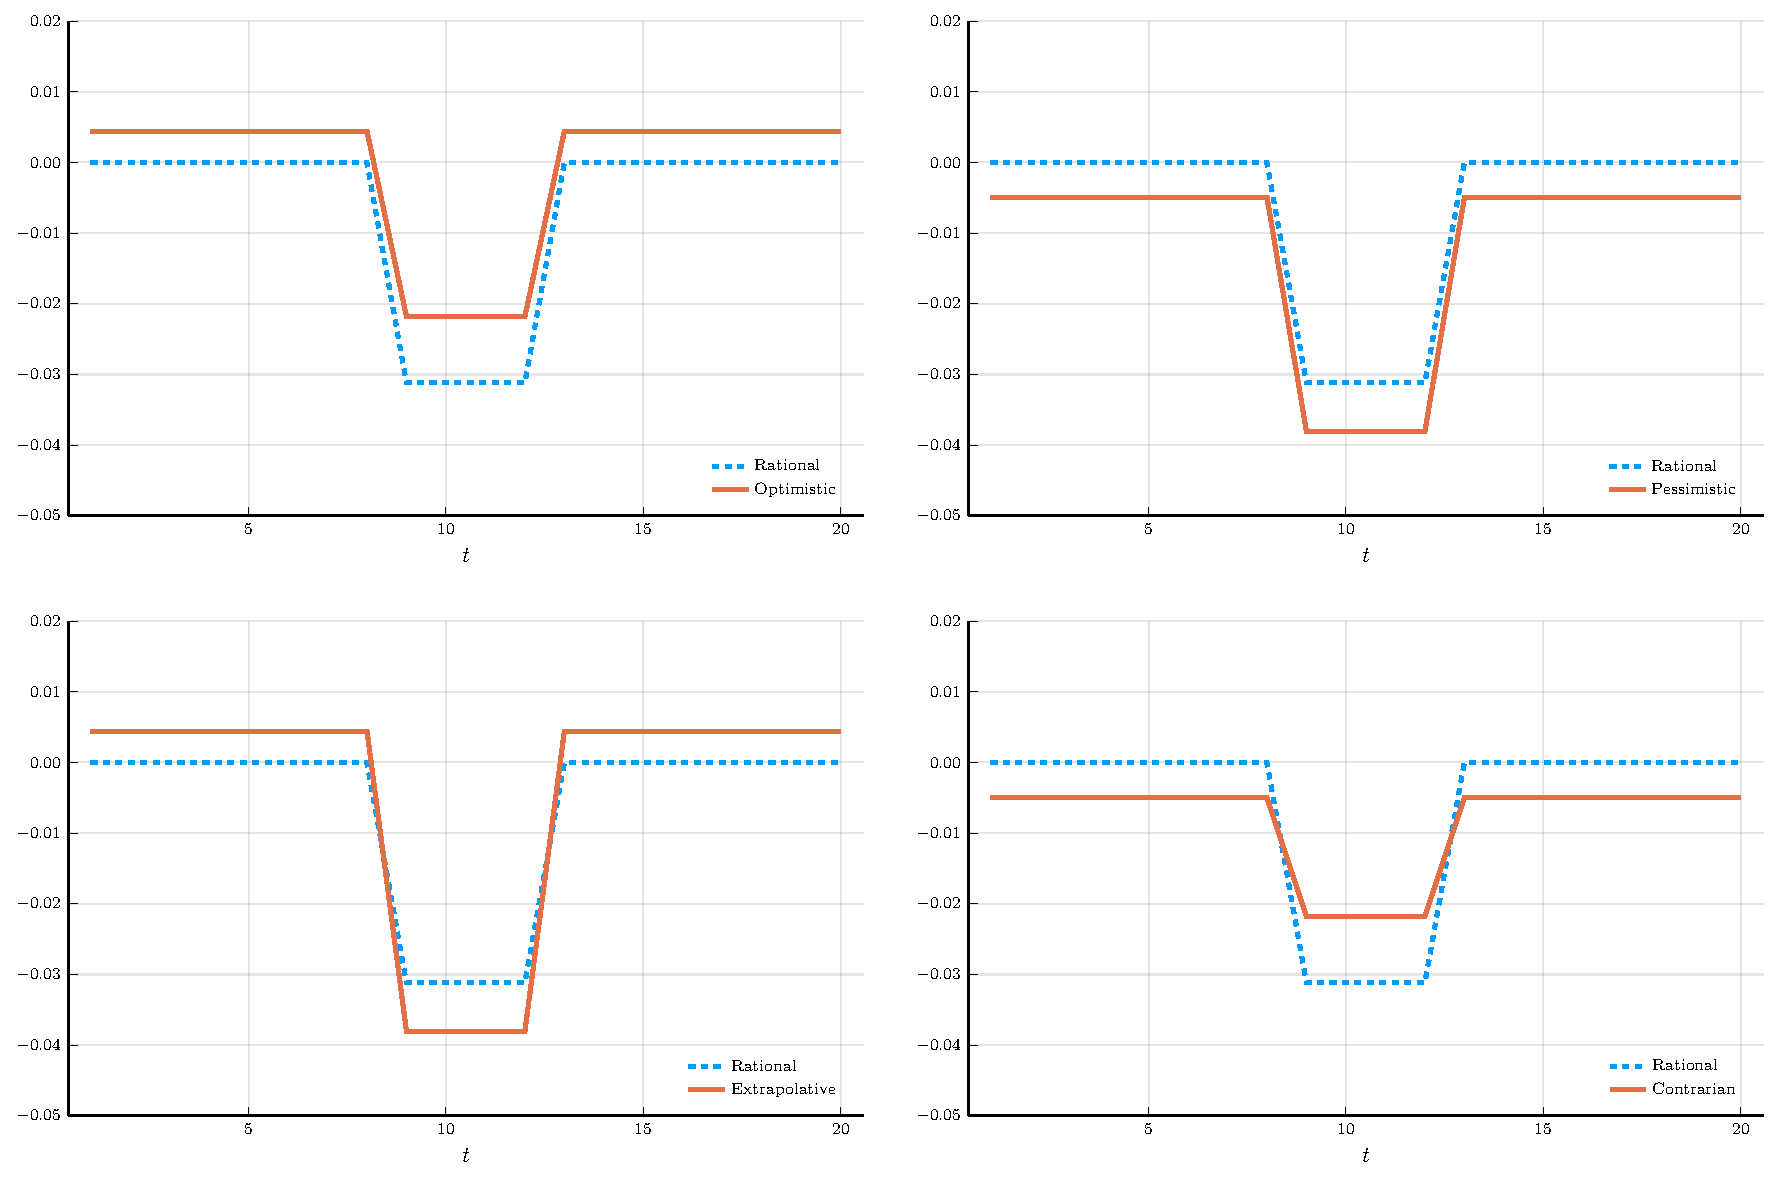
\includegraphics[width=0.90
            \textwidth]{figures/simul_hom_beliefs.pdf}
    \caption{Homogeneous beliefs}
    \caption*{  \scriptsize 
    Note: examples of cycles (four periods of bad shocks with sixteen periods of expansions) with homogeneous beliefs: rational, always optimistic (top-left panel), always pessimistic (top-right panel), extrapolative (bottom-left panel) and intrapolative (bottom-right panel) beliefs. \par} 
    \vspace{0.0cm}
    \label{fig: hom_beliefs}
\end{figure}

%As we argue in Section \ref{sec:quantitative}, a formulation of diagnostic expectations due to \citet{bordalo2018diagnostic} display extrapolation whenever states are persistent. 

\paragraph{Heterogeneous beliefs.} 

Next, we investigate the internal propagation of the model. As we explained earlier, the internal propagation is induced by belief heterogeneity, through its effect on beliefs. From Proposition \ref{prop: dynamics_beliefs}, we deduce that $\eta_i'(X,s,H) > \eta_i$ if and only if investor $i$ is optimistic at $(X,s)$ relative to market beliefs. We know that optimists' wealth increases after good shocks and decreases after bad shocks. This observation is key to understand the internal propagation of the economy: 
% sb: i'M a bit confused about this item. In turn, we know that \todo{check}$\bar{p}^M_{HH}(X') \geq \bar{p}^M_{sH}(X)$ and $\bar{p}^M_{LH}(X') \leq \bar{p}^M_{sH}(X)$. Thus, market beliefs become more optimistic the optimistic more exposed to risk.

\begin{corollary}\label{cor:het_dynamics} If beliefs are heterogeneous, then:

\begin{itemize}
    \item As the current state persists, the LDF increases (decreases) with time if the current state is high (low) growth.
    \item Consider an initial state $(X,H)$ and a first switch from $s=H$ to $s'=L$ at some future date. Then,
\begin{itemize}
\item If beliefs are \underline{rank-preserving}, the later the date of the switch in the state, the lower the reduction in output (the longer the boom, the lesser the bust). 
%and let $\tilde{X} = \chi(X,H,H)$. If beliefs are rank-preserving, then
%\begin{equation}
%p_{LH}(\chi(\tilde{X},H,L)) > p_{LH}(\chi(X,H,L)),
% \sum_{i=1}^I \eta_i' \frac{p_{HL}^i}{p_{HL}(X')} p_{LH}^i > \sum_{i=1}^I \eta_i \frac{p_{HL}^i}{p_{HL}(X)} p_{LH}^i, \nonumber
%\end{equation}
% where $\eta_i' = \eta_i \frac{p_{HH}^i}{p_{HH}(X)}$, so market beliefs are more optimistic when transitions from $s = H$ to $s' = L$ are delayed.
%so market beliefs are more optimistic when transitions from $s = H$ to $s' = L$ are delayed.

\item  If beliefs are \underline{rank-alternating}, the later the date of the switch in the state (the longer the boom), the lower the reduction in output  (the longer the boom, the greater the bust).
%The longer the state persists, the greater the reduction in output when the state switches from $s=H$ to $s^{\prime}=L$. 
%then
%\begin{equation}
%p_{LH}(\chi(\tilde{X},H,L)) <  p_{LH}(\chi(X,H,L)), \nonumber
%\end{equation}
% \begin{equation}
% \sum_{i=1}^I \eta_i' \frac{p_{HL}^i}{p_{HL}(X')} p_{LH}^i < \sum_{i=1}^I \eta_i \frac{p_{HL}^i}{p_{HL}(X)} p_{LH}^i, \nonumber
% \end{equation}
% so market beliefs are more pessimistic when transitions from $s = H$ to $s' = L$ are delayed.
\end{itemize}
\end{itemize}

\end{corollary}
\begin{proof}
See Appendix \ref{app: proof_cor_het_dynamics}.
\end{proof}
With belief heterogeneity, the economy evolves even without changes in TFP growth. The reason is the joint evolution of wealth and market beliefs. From Proposition \ref{prop: dynamics_beliefs}, optimists' wealth share increases while the economy is in a boom. Market beliefs become more optimistic relative to rational expectations as optimists accumulate wealth. This force leads to increased labor demand throughout during the boom. The converse is true during a low growth phase: pessimists accumulate wealth and market beliefs tilt toward greater pessimism.

\begin{figure}[t!]
    \centering
            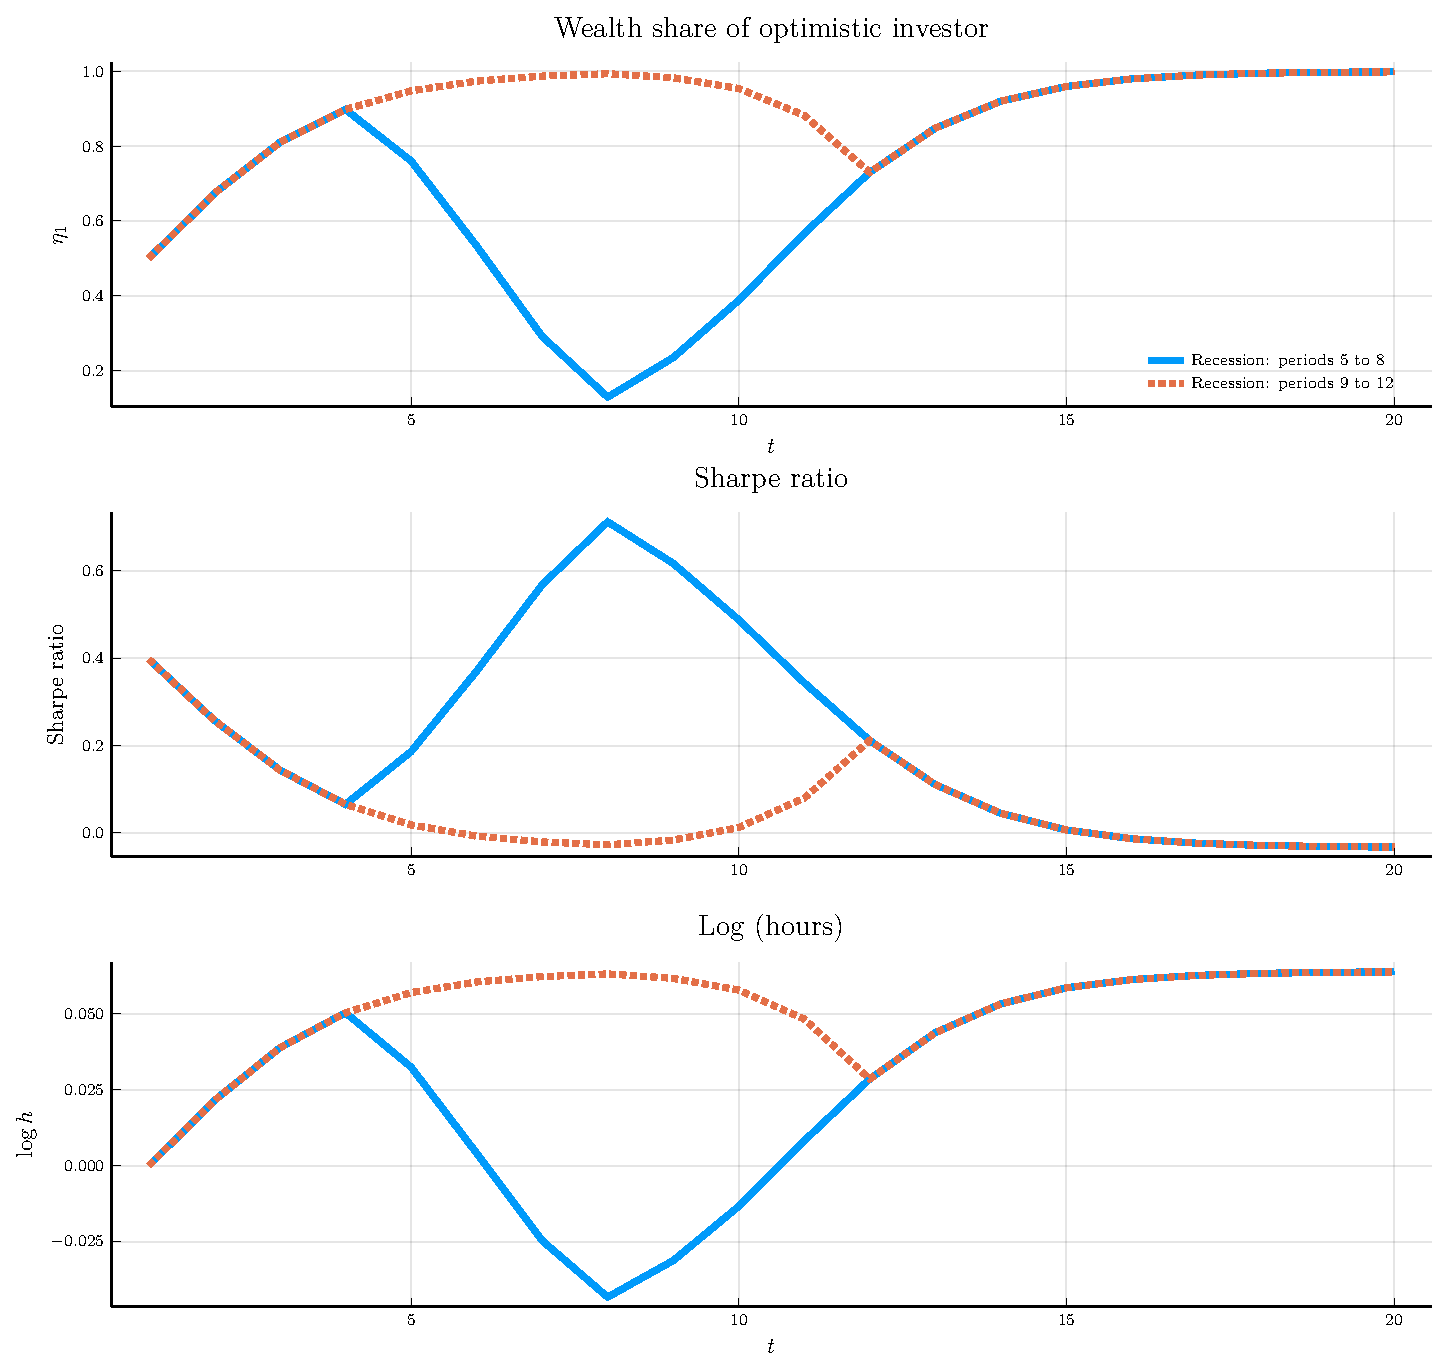
\includegraphics[width=0.75
            \textwidth]{figures/simul_het_beliefs1.pdf}
    \caption{Heterogeneous beliefs: optimistic vs pessimistic}
    \caption*{  \scriptsize 
    Note: examples of cycles (four periods of bad shocks with sixteen periods of expansions) with heterogeneous beliefs: $I=2$ investors, always optimistic and always pessimistic. The top panel shows the wealth share of the optimistic investor, the middle panel shows the Sharpe ratio (under objective beliefs), and the bottom panel shows log labor hours. \par} 
    \vspace{0.0cm}
    \label{fig: het_beliefs1}
\end{figure}

The connection between the length of cycles and their amplitude (the drop in output after a change in state) crucially hinges on whether beliefs are rank-preserving or rank-alternating. 
Rank-preserving beliefs attenuate the subsequent decline in TFP growth in a recession that follows a longer boom. 
The relationship between the duration of the high-growth phase and the severity of the recession is reversed with rank-alternating beliefs.

Figure \ref{fig: het_beliefs1} aids us to explain this pattern. The figure shows simulations of business cycles in the case of rank-preserving beliefs---the figure uses $I=2$, where investor 1 is optimistic and investor 2 is pessimistic in both states. The figure shows the evolution of the wealth share of the optimist, the Sharpe ratio, and log hours. The lower panel shows that the drop in hours is smaller as the economy remains longer in the high state. 
As optimists accumulate wealth during the high-growth phase. Their accumulate wealth implies that, when the economy switches states, optimists arrive at the bad state with more wealth, the longer the boom. Since optimists remain optimistic during downturns when beliefs are rank preserving, their greater wealth makes market beliefs more optimistic during crashes. This rank-preservation attenuates the increase in risk premia and the decline in hours. 

Figure \ref{fig: het_beliefs2}, is the analogue figure for rank-alternating beliefs---investor 1 is rational and investor 2 is extrapolative. The top panel shows that the wealth share of the rational investor declines during the boom phase. This means that extrapolative investors are getting wealthier as the boom lasts longer. Consequently, extrapolative households have a larger wealth share during busts, precisely when they become pessimistic. As a result, market beliefs become more pessimistic after the economy transitions to a low state when beliefs are extrapolatve. Belief extrapolation amplifies the increase in risk-premia and the decline in hours.


\begin{figure}[t!]
    \centering
            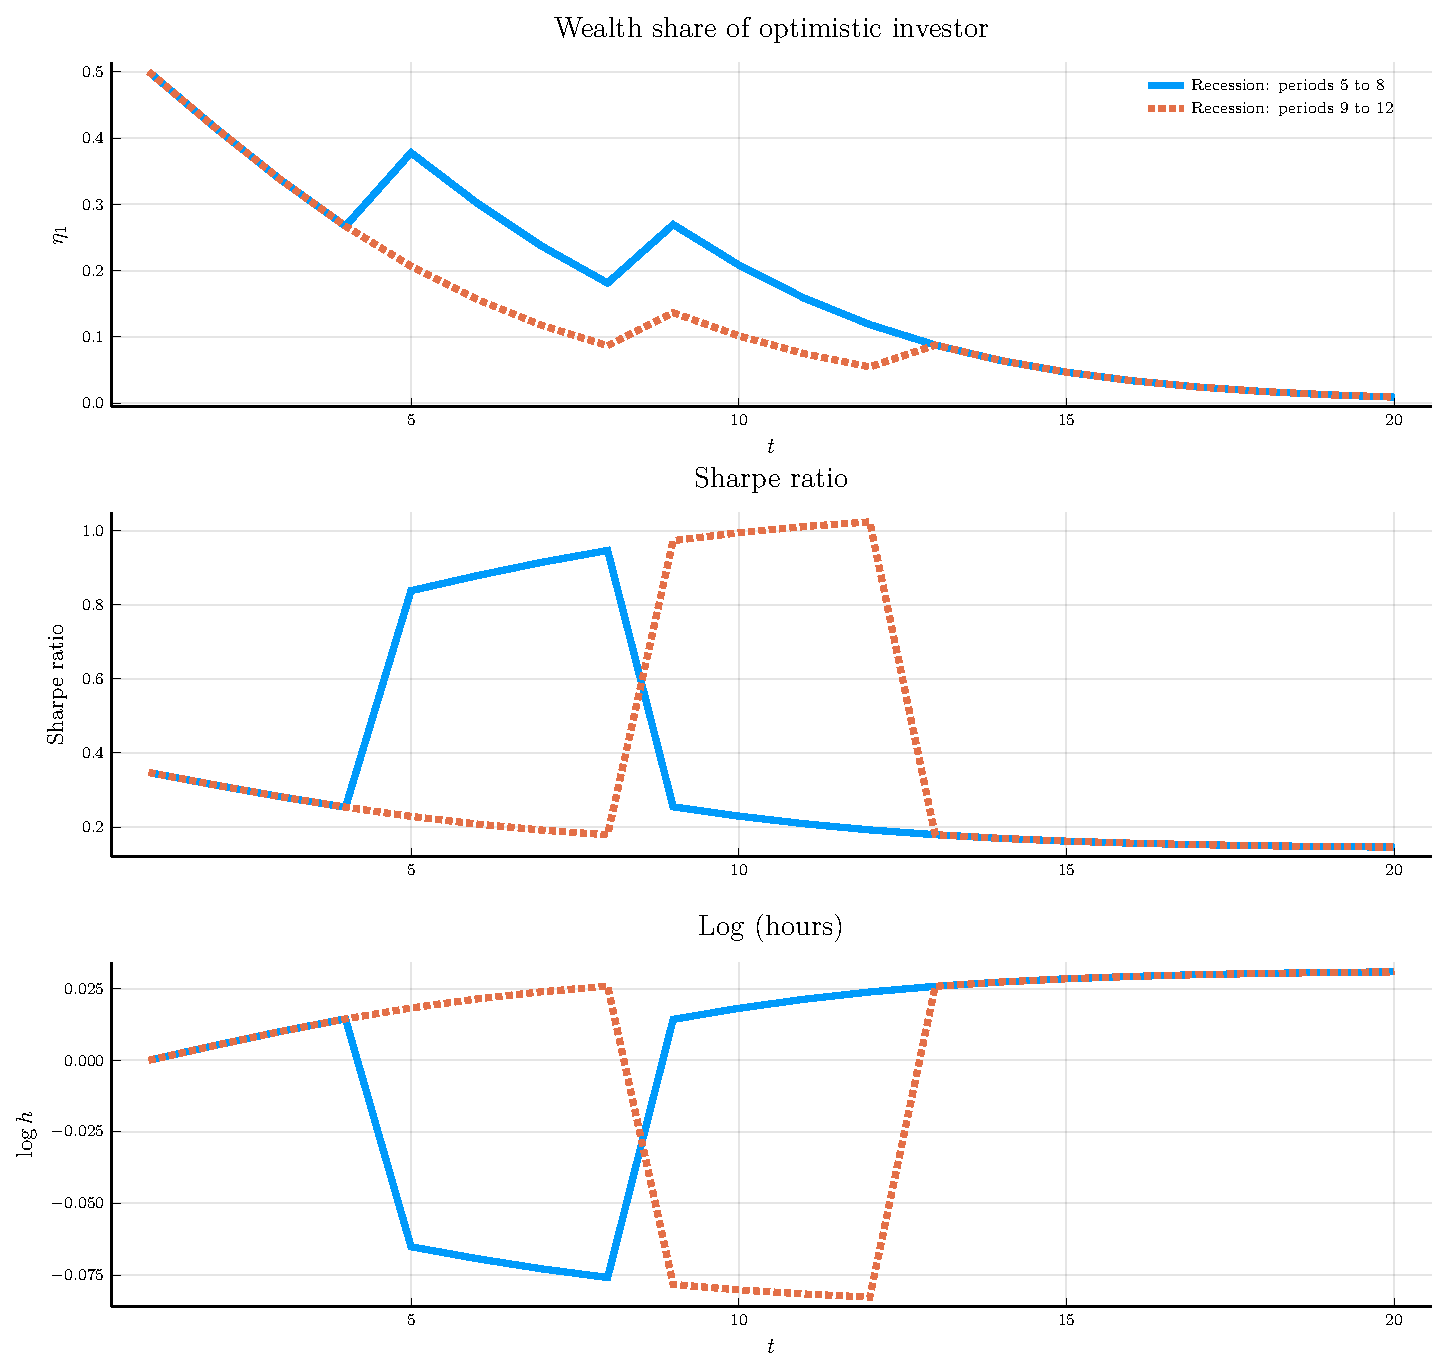
\includegraphics[width=0.75
            \textwidth]{figures/simul_het_beliefs2.pdf}
    \caption{Heterogeneous beliefs: rational vs extrapolative}
    \caption*{  \scriptsize 
    Note: examples of cycles (four periods of bad shocks with sixteen periods of expansions) with heterogeneous beliefs: $I=2$ investors, rational and extrapolative. The top panel shows the wealth share of the optimistic investor, the middle panel shows the Sharpe ratio (under objective beliefs), and the bottom panel shows log labor hours. \par} 
    \vspace{0.0cm}
    \label{fig: het_beliefs2}
\end{figure}

\paragraph{Frothy markets and risk build-ups.} An implication of Corollary \ref{cor:het_dynamics} is that the risk premium declines with the length of economic expansions. 
% If we think that real-world credit spreads, which are not present in the model, are partly driven by risk premium, 
To the extent that credit spreads are driven by risk premia, 
the model's prediction is also consistent with the discussions in \citet{lopez2017credit} and \citet{krishnamurthy2017credit} that argue that economic booms are characterized by "froth" market conditions driven by credit-market \textit{sentiments}.
%In our setting, an increase in average market optimism shifts up the demand for risky assets ultimately compressing spreads. 
%Therefore, the model generates endogenous movements in risk appetite or sentiment.
Moreover, with belief extrapolation, an increase in optimism leads not only to a reduction in risk premia but also an increase in volatility, as shown in Figure \ref{fig: risk_eq}. Under this interpretation, there is endogenous \textit{risk build-up} during booms. 
As argued by \citet{krishnamurthy2020dissecting}, the combination of risk build-up and low spreads is challenging to generate for standard macro-finance models, such as \citet{he2013intermediary} and \citet{brunnermeier2014macroeconomic}. This observation suggests that heterogeneous extrapolative beliefs may explain credit and asset-market dynamics during boom-bust cycles.  

\paragraph{Discussion: belief heterogeneity vs. risk aversion belief.} 
As discussed above, rank-alternating beliefs amplify inherent economic fluctuations.
Therefore, it is not only differences in investors' risk appetite that matters for business cycles, but also how differences in the propensity to take risk to react to shocks. 
For instance, models of heterogeneous risk aversion are able to generate dispersion in portfolios and time variation in expected returns, but the ranking of agents in terms of risk-taking is always the same.
This property is analogous to the case of rank-preserving beliefs shown in Figure \ref{fig: het_beliefs1}.
In contrast, there is no counterpart to the rank-alternating beliefs with heterogeneous risk aversion, as the least risk-averse agent in the boom is also the least risk-averse agent in the bust.
Thus, different forms of investor heterogeneity have different implications for business cycle fluctuations, asset prices, and trading.


\subsection{Trade Volume}

We now consider the implications of heterogeneous beliefs regarding stock turnover, a measure of trading volume. To compute the stock turnover, we first map the portfolio holdings of the surplus claim, $\omega_i$, into the effective number of shares on firm equity in the primitive economy. This mapping is straightforward in the case of linear labor disutility, $\nu = 0$ because human wealth is zero in this case.\footnote{The share of wealth invested in stocks is $\omega_i$, given that human wealth is equal to zero, $\mathcal{H}_i = 0$, and $R_{e}(X,s,s') = R_{r}(X,s,s')$ under this assumption.} To simplify the exhibition, we adopt this assumption for the rest of the section. The traded volume in this case is:
% \footnote{The portfolio share is given by $\omega_{i,t} \equiv \frac{Q_t S_{i,t}}{N_{i,t}(1-c_{i,t})} $, so $S_{i,t} = \frac{\omega_{i,t} N_{i,t} (1-c_{i,t})}{Q_t}$. Given $1-c_{i,t} = \beta$ and $Q_t = \beta P_t$, assuming $\nu = 0$, we obtain $\mu_{i,t} S_{i,t} = \frac{\omega_{i,t} \mu_i N_{i,t}}{P_t} = \omega_{i,t} \eta_{i,t} $. Shares traded by type-$i$ investors are $\mu_{i,t} |S_{i,t}- S_{i,t-1}| = |\omega_{i,t}\eta_{i,t} - \omega_{i,t-1} \eta_{i,t-1}|$.}
\begin{equation}
    \tau_t = \frac{1}{2} \sum_{i=1}^I |\omega_{i,t} \eta_{i,t} - \omega_{i,t-1} \eta_{i,t-1} |.\nonumber
\end{equation} 
% Trading volume, or equivalently turnover as the number of shares is normalized to one, depends on the degree of belief heterogeneity. 
This formula shows that the volume traded depends on the level of disagreement. 

We consider a small deviation from homogeneous beliefs to study the effect of belief dispersion on volume. We express investor $i$'s beliefs as follows
\begin{equation}
    p_{ss'}^i = p_{ss'}^* + \delta_{ss'}^i \epsilon,\nonumber
\end{equation}
where $\delta_{sH}^i + \delta_{sL}^i = 0$ and $\epsilon$ captures belief heterogeneity as discussed earlier. Also, for parsimony, set $p_{ss'}^* = \frac{1}{2}$, such that, in the absence of heterogeneity, beliefs are iid and symmetric---the proofs in the Appendix hold for general common belief case.
%let's assume beliefs are iid for $\epsilon = 0$, $p_{sH}^* = p_{sL}^*$.\todo{this is not i.i.d. I.i.d is the opposite no?}

% Notice that average beliefs in the state $(X,s)$ is the same for both economies, as $\sum_{i=1}^I \eta_i p_{ss'}^i = p_{ss'}^*$, so moving from $\epsilon = 0$ to $\epsilon > 0$ increases the dispersion in beliefs, keeping the average probability of a given state constant.
The portfolio share of investor $i$ is:
\begin{equation}
    \omega_{i}(X,s; \epsilon) = 1 +\kappa_\omega \left[p_{sH}^i - \overline{p}^m_{sH}(X)\right] + \mathcal{O}(\epsilon^2),\nonumber
\end{equation}
where $\kappa_\omega$ is a positive constant. This expression showcases how optimistic investors, for whom $p_{sH}^i > \overline{p}^m_{sH}(X)$, are long in stocks. 

Consider current and future states $s$ and $s'$. The effect of a perturbation in $\epsilon$ on the trades of investor $i$ is:
\begin{equation}\label{eq: trading}
    \Delta S_i(X,s,s';\epsilon) =
    \underbrace{\Delta \eta_i(X,s,s')}_{\text{rebalancing effect}}+\underbrace{\Delta \omega_i(X,s,s') \eta_i}_{\text{change-in-beliefs effect}} + \mathcal{O}(\epsilon^2),
\end{equation}
as the economy switches from state $(X,s)$ to $(X',s')$, where 
%$\tilde{\delta}_{ss'}^i \equiv \delta_{ss'}^i - \delta_{ss'}(X)$ and 
\begin{align}
    \Delta \eta_i(X,s,s') \equiv \eta_i \frac{p_{ss'}^i - \overline{p}_{ss'}^m(X)}{p_{ss'}^*} , \qquad
    \Delta \omega_i(X,s,s') &\equiv \kappa_\omega\left[p_{s'H}^i - \overline{p}_{s'H}^m(X) - (p_{sH}^i - \overline{p}^m_{sH}(X)) \right] .\nonumber
\end{align}
The expression \eqref{eq: trading} reveals two effects: The \textit{rebalancing effect} captures the extent to which investors trade after a change in the state to keep portfolio shares constant: investors who put more likelihood on the realized state relative to the market belief, increased (decreased) their wealth share. Thus, they must buy (sell) the risky asset when that state is realized, to keep the portfolio share constant. Of course, as the economy evolves from $s$ to $s'$, portfolio shares themselves change as beliefs are modified. The \textit{change-in-beliefs effect} captures the trade that follows the change in portfolio shares as the state changes. The change-in-beliefs effect equals zero if $s = s'$, as individual beliefs are constant.  

In tandem, the effects of rebalancing and change-in-beliefs determine equilibrium turnover. 
\begin{proposition}[Turnover]\label{prop: turnover} 
% Let $\eta_o = \sum_{i=1}^I \eta_i \textbf{1}_{\delta_{sH}^i >0}$  denote the share of wealth of optimists and $\eta_p = \sum_{i=1}^I \eta_i \textbf{1}_{\delta_{sH}^i \leq 0}$ the share of wealth of pessimists. Similarly, define $\delta_{sH}^o = \frac{1}{\eta_o} \sum_{i=1}^I \eta_i \delta_{s H}^i \textbf{1}_{\delta_{s H}^i  >0 }$  and $\delta_{sH}^p = \frac{1}{\eta_p} \sum_{i=1}^I \eta_i \delta_{s H}^i \textbf{1}_{\delta_{s H}^i \leq 0}$. 
The economy's turnover, as it switches from state $(X,s)$ to state $(X',s')$, is given by
\begin{equation}\label{eq: turnover}
    \tau(X,s,s';\epsilon) = \frac{1}{2} \sum_{i=1}^I \eta_i\left\lvert  \frac{p_{ss'}^i - \overline{p}_{ss'}^m(X)}{p_{ss'}^*} +\kappa_\omega\left[p_{s'H}^i - \overline{p}_{s'H}^m(X) - (p_{sH}^i - \overline{p}^m_{sH}(X)) \right] \right\rvert  + \mathcal{O}(\epsilon^2).
\end{equation}
\end{proposition}
\begin{proof}
See Appendix \ref{app: proof_cor_het_dynamics}.
\end{proof}

Proposition \ref{prop: turnover} provides a characterization of turnover. When $s = s'$, the change-in-beliefs effect vanishes; turnover is driven solely by the rebalancing effect:
\begin{equation}
    \tau(X,s,s';\epsilon) = \frac{1}{2} \sum_{i=1}^I \eta_i \frac{|p_{ss'}^i - \overline{p}_{ss'}^m(X)|}{p_{ss'}^*} + \mathcal{O}(\epsilon^2).\nonumber
\end{equation}
Thus, when there is no change in the state of the economy,  turnover is proportional to the average absolute deviation of beliefs. The formula is consistent with the evidence in Section \ref{sec:mechanism}, which shows that dispersion on subjective beliefs about cash flows is correlated with stock market turnover.  
% This expression is the analogous in our two-state setting of the empirical specification adopted in Section \ref{sec:facts.sec}.

The change-in-beliefs effect emerges when the economy switches states, that is, when $s \neq s'$. This effect may either amplify or dampen the rebalancing effect, depending on the type of belief and the direction of change in the economy. For instance, suppose that $s = H$ and $s' = L$ and beliefs are rank-alternating. Optimistic investors lose wealth as the economy switches to a bad state. The rebalancing effect implies that they must sell some risky assets to maintain their portfolio shares once stocks lose value. These investors also become pessimists in downturns, leading them to sell even more stocks. Thus, the two effects go in the same direction, amplifying the impact on the turnover when the economy switches from high to low states. The two effects are opposite when $s = L$ and $s' = H$. Pessimists become optimistic as the economy switches to the high state, which induces them to increase their stock portfolio share. At the same time, the rebalancing effect dictates that they sell stocks once stocks appreciate to keep the portfolio balanced.

\paragraph{Connecting with the Turnover Evidence.}\todo{have not reviewed.}
It is convenient to express heterogeneity in beliefs, $p_{ss}^i$, in terms of heterogeneity in the perceived \textit{persistence} of fundamentals. Assuming investors agree on the unconditional mean of $x_t$, $\overline{x}$, we can write $\mathbb{E}_{i,t}[x_{t+1}] - \overline{x} = \theta_i (x_t - \overline{x})$, where $\theta_i$ is a function of $p_{ss'}^i$.
% We can recast beliefs about $p_{ss}^i$ into beliefs about mean reversion rates in earning growth, $\theta^i$---as estimated in Section \ref{sec:quantitative}. 
The following corollary shows heterogeneous beliefs lead to larger turnover rates as the economy switches from booms to recessions.
\begin{corollary}\label{cor: turnover} Suppose investors agree on the unconditional mean of $x_t$, i.e. $p_{LH}^i / p_{HL}^i = \overline{p}_H / \overline{p}_L$ and that the following condition is satisfied: $p_{ss'}^* = \overline{p}_H = \frac{1}{2}$. Turnover as the economy switches from $s$ to $s'$ is given by
\begin{equation}
    \tau(X,H,L;\epsilon) = \frac{\zeta(s,s')}{2}\sum_{i=1}^I \eta_i |\theta_i - \theta(X)| + \mathcal{O}(\epsilon^2),
\end{equation}
where
\begin{equation*}
    \zeta(s,s') \equiv \left\{ 
    \begin{matrix}
    \kappa_\omega + 1, \qquad & \text{if } $s = H$ \text{ and } $s' = L$\\
    |\kappa_\omega - 1|, \qquad & \text{if } $s = L$ \text{ and } $s'  = H$\\
    1, \qquad & \text{if } $s = s'$
    \end{matrix}
    \right. 
\end{equation*}
\end{corollary}
% The assumption $p_{ss'}^* = \overline{p}_H = \frac{1}{2}$ is made only to simplify the presentation. The general case is considered in the appendix.
 The key message from Corollary \ref{cor: turnover} is that turnover increases in belief dispersion and, furthermore, that the effect is more pronounced during busts. 
Both predictions are in line with the evidence discussed in Section \ref{sec:mechanism}. The assumption of rank-alternating beliefs is important to obtain this asymmetric effect. 
If investors have rank-preserving beliefs, where they are equally optimistic or pessimistic in both states, so $\tilde{\delta}_{s'H}^i = \tilde{\delta}_{sH}^i $ even for $s'\neq s$, then the change-in-beliefs effect will be equal to zero and we would not obtain a stronger response of turnover to disagreement during bad times. Therefore, rank-alternating beliefs are key to capturing the dynamics of stock market turnover. 

% Moreover, differences in $\delta_{ss'}^i$ can be recast into differences in the persistence of cash-flows, as in our empirical specification.
